\chapter{بناء نموذج عملي وربطه بالنماذج الأخرى}
\label{ch:04-forms}
\section{خطّط النموذج قبل بنائه}
\label{sec:forms-plan}
قبل فتح المنشأة اكتب على ورقة ثلاثة أشياء: ماذا نريد أن نعرف، وعن أي منشأة، وما القواعد التي تمنع الإجابة الخاطئة. هذا يوفر عليك إعادة البناء لاحقاً.

\begin{rcnote}[تطبيق المثال: خطة نموذج «بيانات التشغيل»]
نريد معرفة عدد العاملين وأيام التوقف وسببه في مصنع الأفق خلال أيلول 2026. يرتبط النموذج بسجل المنشأة، وفيه صفحتان: «المنشأة والفترة» و«التشغيل».
\end{rcnote}

\begin{table}[H]
\centering
\caption{أسئلة نموذج «بيانات التشغيل»}
\label{tab:forms-plan}
\begin{tabularx}{\linewidth}{R{2.6cm} R{2.8cm} Y}
\rcHeaderRow
\thh{السؤال} & \thh{نوعه} & \thh{قاعدته}\\
المنشأة & «اختيار من الكيانات» & مطلوب، ومملوء من التكليف.\\
فترة المسح & «فترة (من – إلى)» & مطلوب: من 1 إلى 30 أيلول 2026.\\
عدد العاملين & «رقم» (الوحدة: عامل) & مطلوب، ولا يقل عن 0.\\
أيام التوقف & «رقم» (الوحدة: يوم) & مطلوب، من 0 إلى 30.\\
سبب التوقف & «اختيار واحد» & يظهر ويصبح مطلوباً عندما تكون أيام التوقف أكبر من 0.\\
\end{tabularx}
\end{table}

خيارات «سبب التوقف» في المثال: انقطاع الكهرباء، نقص المواد الأولية، صيانة، أخرى.

\section{أنشئ النموذج وأضف أسئلته}
\label{sec:forms-create}

\textbf{أنشئ النموذج:}

\begin{enumerate}
\item افتح «ادوات البناء» ثم «الأساسية» ثم «النماذج»، واضغط «إنشاء نموذج».
\item اكتب «اسم النموذج» و«كود النموذج» والوصف، واختر التطبيق وقسمه. لا يمكن تغيير «كود النموذج» بعد الإنشاء، والوصف يحتاج إلى كلمتين على الأقل.
\item اضغط «إنشاء». يفتح «منشئ النماذج» وفيه قسم وسؤال واحد.
\end{enumerate}

\textbf{أضف الصفحات والأسئلة:}

\begin{enumerate}
\item اضغط «إضافة صفحة»، واكتب «عنوان الصفحة» من «إعدادات الصفحة».
\item أضف السؤال من «اختر نوع الحقل»، ثم اكتب نصه.
\item اضغط السؤال لتفتح إعداداته. في سؤال «رقم» حدّد «الحد الأدنى» و«الحد الأعلى»، واكتب الوحدة في «بعد الرقم».
\item في «اختيار واحد» اختر «العرض» «قائمة منسدلة»، واكتب «الخيارات».
\item في سؤال «المنشأة» من نوع «اختيار من الكيانات» اختر «نوع السجل»، ثم فعّل «سؤال سجل». بهذا تعرف الحزمة والخطة المنشأة التي تخصها الإجابة.
\end{enumerate}

\begin{figure}[H]
\centering
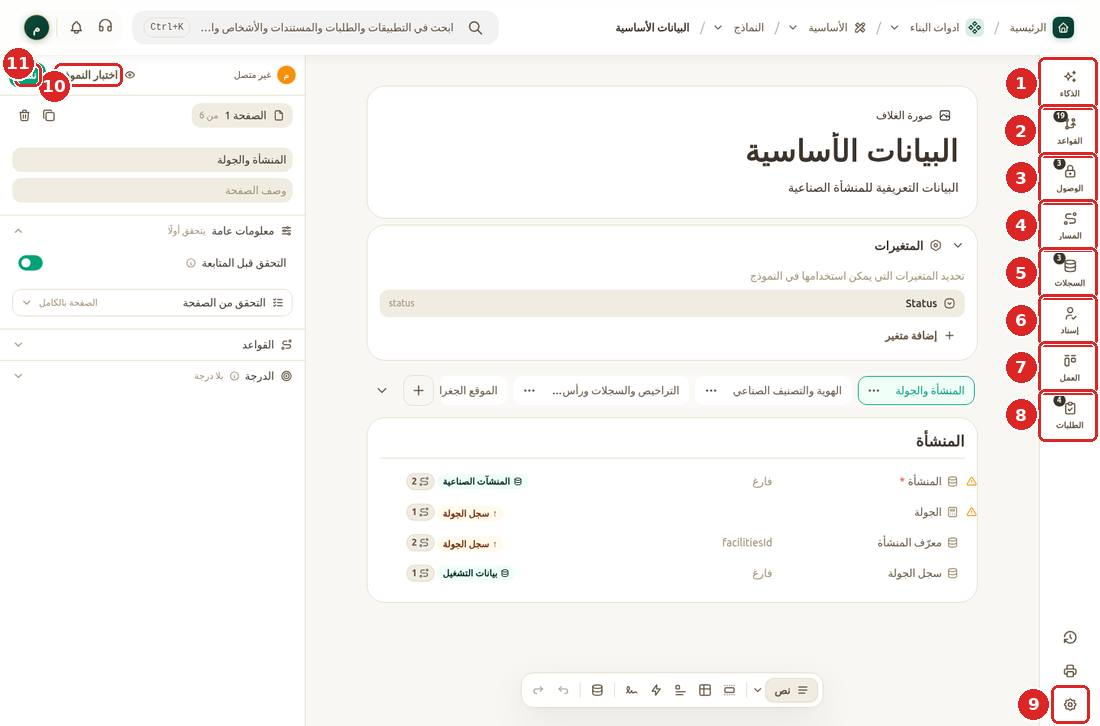
\includegraphics[width=\linewidth]{assets/screens/forms-builder-ar.jpg}
\caption{منشئ النماذج وشريط أدواته}
\label{fig:forms-builder}
\shotnote{هذه شاشة بناء النموذج: الأسئلة في الوسط، وأدوات النموذج في الشريط الجانبي. تفيدك في معرفة مكان كل إعداد قبل أن تبدأ؛ فلكل أداة درج يُفتح منفرداً. لا يصل أي تعديل إلى الباحثين قبل «نشر». ① «الذكاء»: مساعد البناء. ② «القواعد»: الإظهار والإلزام والقفل والقيم والحساب والتحقق. ③ «الوصول»: من يرى ويعبّئ ويراجع. ④ «المسار»: مراحل الموافقة. ⑤ «السجلات»: ما يُكتب في السجلات. ⑥ «إسناد»: التكليف بهذا النموذج. ⑦ «العمل»: الحزمة والخطة. ⑧ «الطلبات»: الإجابات المرسلة. ⑨ الإعدادات. ⑩ «اختبار النموذج». ⑪ «نشر».}
\end{figure}

\begin{rcnote}[تطبيق المثال]
تنشئ سارة النموذج باسم «بيانات التشغيل» وكود \en{ops\_data}. في الصفحة الأولى تجعل «المنشأة» من نوع «اختيار من الكيانات»، وتختار نوع سجل المنشآت، وتفعّل «سؤال سجل». وفي صفحة «التشغيل» تضيف «عدد العاملين» من نوع «رقم»: الحد الأدنى 0، و«بعد الرقم» «عامل». ثم تضيف «أيام التوقف»: من 0 إلى 30، والوحدة «يوم». وأخيراً تضيف «سبب التوقف» قائمة منسدلة بخياراتها الأربعة.
\end{rcnote}

\section{أضف القواعد}
\label{sec:forms-rules}

القاعدة تجعل النموذج يتصرف بحسب الإجابات: يُظهر سؤالاً، أو يجعله مطلوباً، أو يرفض قيمة خاطئة.

\begin{table}[H]
\centering
\caption{أنواع القواعد}
\label{tab:forms-rules}
\begin{tabularx}{\linewidth}{R{3cm} Y}
\rcHeaderRow
\thh{النوع} & \thh{ماذا يفعل؟}\\
«إظهار أو إخفاء» & يُظهر السؤال أو يخفيه بحسب شرط.\\
«إلزام» & يجعل السؤال مطلوباً دائماً، أو عندما يتحقق شرط.\\
«قفل التعديل» & يمنع تعديل السؤال، دائماً أو بشرط.\\
«قيمة افتراضية» & يضع قيمة مبدئية في السؤال.\\
«حساب» & يحسب قيمة من إجابات أخرى.\\
«تحقق» & يرفض القيمة الخاطئة ويعرض رسالة.\\
\end{tabularx}
\end{table}

\textbf{خطوات إضافة قاعدة:}

\begin{enumerate}
\item افتح «القواعد» واضغط «إضافة قاعدة».
\item اختر «نوع القاعدة».
\item اكتب الشرط في «عندما»: السؤال والقيمة.
\item اختر السؤال الذي تطبق عليه القاعدة.
\item جرّبها بإجابات للتجربة في «جرّبها»، ثم احفظ.
\end{enumerate}

\textbf{مستوى رسالة التحقق:} «خطأ» يمنع الانتقال والإرسال. و«تنبيه» يمنع الإرسال حتى يكتب الباحث سبباً. وتوجد أيضاً «ملاحظة للمراجع» و«تلميح».

\begin{figure}[H]
\centering
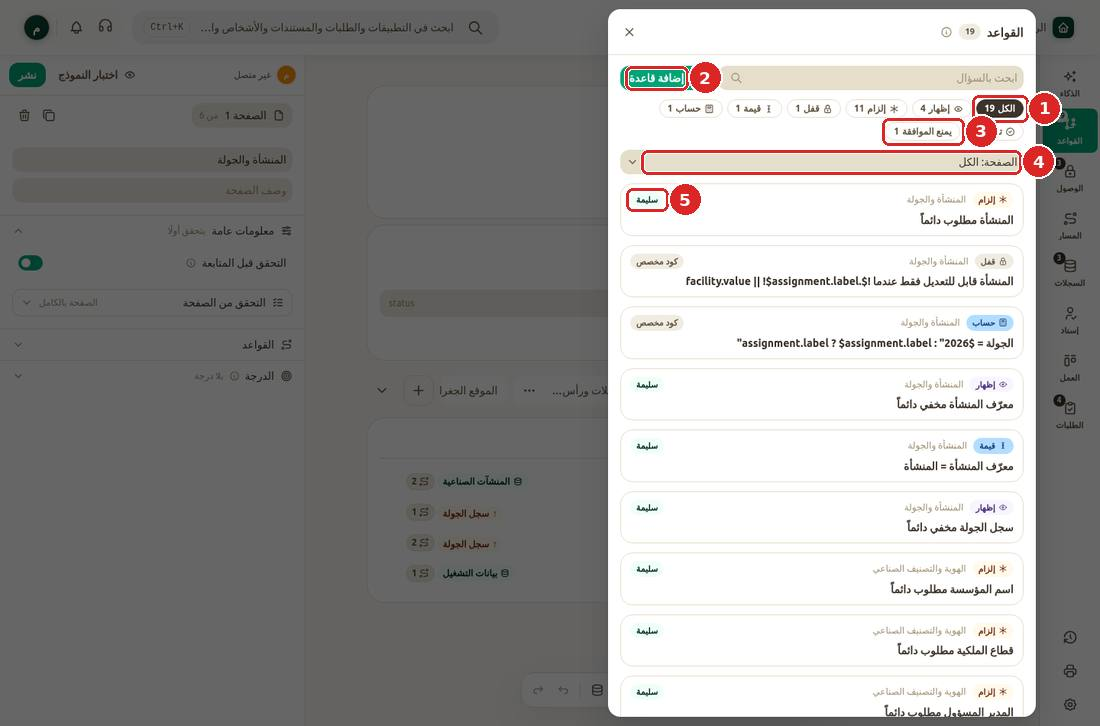
\includegraphics[width=\linewidth]{assets/screens/forms-rules-ar.jpg}
\caption{درج «القواعد» في نموذج قائم}
\label{fig:forms-rules}
\shotnote{يعرض الدرج كل قواعد النموذج في قائمة واحدة، مع نوع كل قاعدة وصفحتها. يفيدك في مراجعة القواعد بعد إضافتها، ومعرفة ما إذا كانت سليمة. ① «الكل» ومرشحات الأنواع: إظهار، إلزام، قفل، قيمة، حساب. ② «إضافة قاعدة». ③ «يمنع الموافقة»: قاعدة تمنع الاعتماد ما دامت مخالفة. ④ «الصفحة: الكل». ⑤ «سليمة»: القاعدة صالحة ومراجعها موجودة.}
\end{figure}

\begin{rcnote}[تطبيق المثال: قاعدتان وثلاث تجارب]
تضيف سارة قاعدة «إظهار أو إخفاء»: يظهر «سبب التوقف» عندما تكون «أيام التوقف» أكبر من 0. ثم قاعدة «إلزام» بالشرط نفسه. وتجربهما في «جرّبها»:
\begin{itemize}
\item أيام التوقف = 3: يظهر «سبب التوقف» ويصبح مطلوباً.
\item أيام التوقف = 0: يختفي السؤال، ولا يُطلب.
\item أيام التوقف = 40: تظهر رسالة «خطأ»، لأن الحد الأعلى 30، ولا يستطيع عمر الإرسال.
\end{itemize}
\end{rcnote}

\section{اربط النموذج بسجل المنشأة}
\label{sec:forms-records}

الربط يجعل النموذج يقرأ من ملف المنشأة ويكتب فيه. يُضبط من «السجلات» أو من «السجل» في إعدادات السؤال.

\begin{itemize}
\item \textbf{«الاتجاه»:} «قراءة» أو «كتابة» أو «قراءة وكتابة».
\item \textbf{«التعبئة المسبقة»:} تملأ الإجابة من السجل قبل أن يبدأ الباحث.
\item \textbf{وقت الكتابة:} «عند الاعتماد» هو الأنسب للمسح، فلا يتغير الملف قبل آخر توقيع.
\item \textbf{«عند التعارض»:} ماذا يحدث إذا تغيّر السجل بعد بدء الإجابة: «إبقاء قيمة السجل» أو «الكتابة فوقها» أو «السؤال عند الاعتماد».
\item \textbf{صلاحية الكتابة:} القراءة تعمل فوراً. أما الكتابة فتحتاج إلى موافقة مسؤول نوع السجل؛ اضغط «طلب الصلاحية».
\end{itemize}

\begin{figure}[H]
\centering
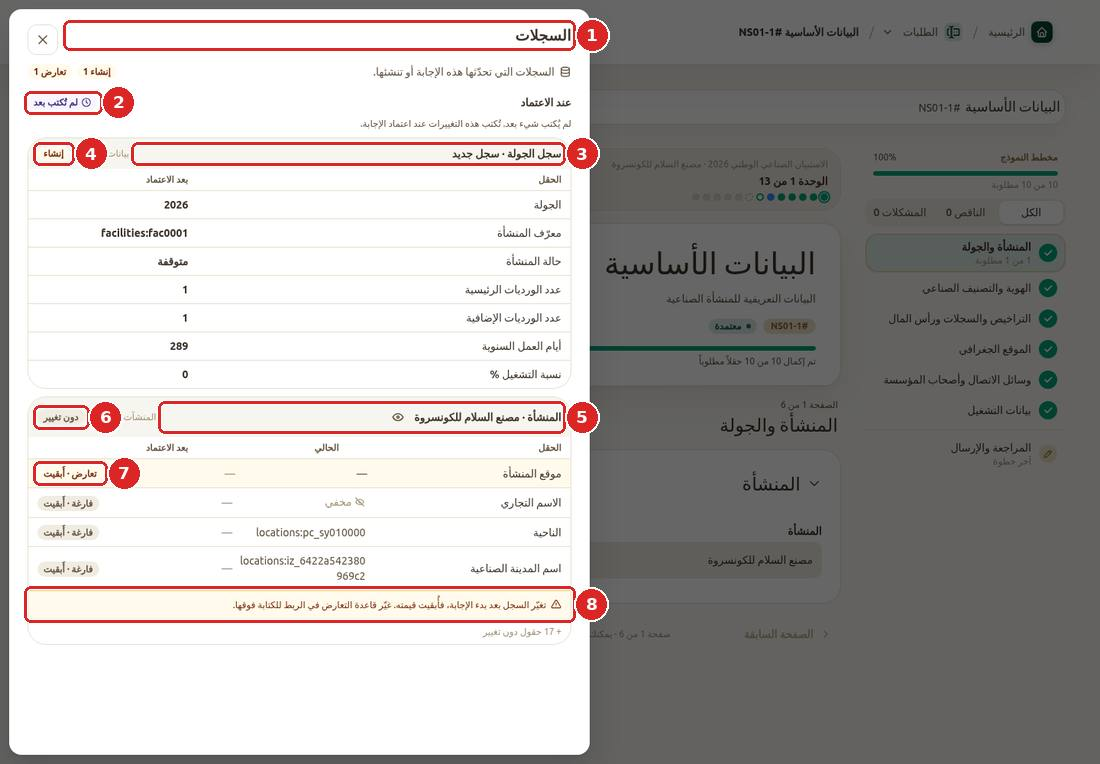
\includegraphics[width=\linewidth]{assets/screens/forms-records-ar.jpg}
\caption{لوحة «السجلات» في إجابة لم تُعتمد بعد}
\label{fig:forms-records}
\shotnote{تبيّن اللوحة ما ستكتبه الإجابة في السجلات عند اعتمادها، قبل أن يحدث ذلك. تفيدك في التأكد من أن الربط صحيح: أي سجل سيُنشأ، وأي حقل سيتغير، وأي قيمة ستبقى. ① «السجلات». ② «لم تُكتب بعد»: الكتابة تتم عند الاعتماد. ③ «سجل الجولة · سجل جديد». ④ «إنشاء». ⑤ سجل المنشأة. ⑥ «دون تغيير». ⑦ «تعارض · أُبقيت»: تغيّر السجل بعد بدء الإجابة فأُبقيت قيمته. ⑧ شرح التعارض وطريقة تغييره.}
\end{figure}

\begin{rcnote}[تطبيق المثال]
يقرأ سؤال «المنشأة» ملف مصنع الأفق، فيظهر اسمه مملوءاً ومقفلاً. ويكتب «عدد العاملين» و«أيام التوقف» و«سبب التوقف» في سجل جولة أيلول 2026 «عند الاعتماد». تطلب سارة صلاحية الكتابة، ويوافق مسؤول نوع السجل.
\end{rcnote}

\section{حدّد الوصول والمسار ثم اختبر وانشر}
\label{sec:forms-publish}

\textbf{الوصول:} من «الوصول» حدّد من يبدأ النموذج ومن يراجعه.

\textbf{المسار:} من «المسار» اضغط «تفعيل المسار». افعل ذلك في كل نموذج يدخل حزمة، حتى لو لم تكن فيه موافقات؛ فبدونه لا يظهر للباحث زر «إرسال الوحدة». ثم فعّل «خطوات الموافقة»، وأضف «خطوة موافقة» واحدة فيها مرحلة لكل مراجع بالترتيب. نشرح حقول الخطوة كلها في القسم~\ref{sec:review-setup}. وضع أسئلة كل صفحة داخل قسم، وإلا لم يستطع المراجع تقييمها.

\textbf{الاختبار:} اضغط «اختبار النموذج»، واختر عضواً، ثم «بدء الاختبار». تعمل التجربة في مساحة «معزولة» لا تؤثر في البيانات الحقيقية، وتتصرف بصفة العضو الذي اخترته.

\textbf{النشر:} اضغط «نشر»، وراجع «ما الذي سيتغيّر»، واكتب ملاحظة التغيير، ثم أكّد. الإجابات المفتوحة تبقى على إصدارها القديم، والجديدة تستخدم الإصدار الجديد.

\begin{rcnote}[تطبيق المثال]
تضيف سارة خطوة موافقة واحدة بأربع مراحل: تدقيق آلي، ثم ليلى، ثم خالد، ثم رنا. تختبر النموذج بصفة عمر، وتجرب أيام التوقف 3 ثم 0 ثم 40. وبعد نجاح التجارب الثلاث تضغط «نشر».
\end{rcnote}

\section{أضف النموذج المساعد واجمعهما في حزمة}
\label{sec:forms-package}

\textbf{النموذج المساعد} صغير ويكمل الأول. في مثالنا «متابعة الاحتياج» فيه سؤالان: «نوع الاحتياج» («اختيار واحد») و«وصف الاحتياج» («نص»). يُبنى بالخطوات نفسها، ويحتاج أيضاً إلى سؤال «المنشأة» مع «سؤال سجل»؛ وإلا نبّهت الحزمة: «لا سؤال في نموذج هذه الوحدة لنوع سجل الحزمة».

\textbf{الحزمة} تجمع النماذج لتُكلَّف وتُتابع عملاً واحداً لكل منشأة. أنشئها من «حزمة نماذج جديدة»، ثم أضف النماذج وحداتٍ بالزر «إضافة وحدة». لكل وحدة إعدادات:

\begin{itemize}
\item \textbf{«مطلوبة»:} لا تكتمل الحزمة إلا بها.
\item \textbf{«تُفتح»:} مع بداية الحزمة، أو بعد إرسال وحدة سابقة.
\item \textbf{«وفقط إذا»:} «دائماً» أو «شروط». الوحدة الشرطية تُتخطّى إذا لم يتحقق شرطها.
\item \textbf{«الموعد»:} أيام من فتح الوحدة، ولا يتجاوز موعد الحزمة.
\item \textbf{«عند رفضها»:} «تستمر الحزمة» أو «تتوقف الحزمة».
\end{itemize}

\textbf{طريقة الفتح:} «بالترتيب» تفتح كل وحدة بعد إرسال السابقة. و«معاً» تفتح الوحدات كلها مع البداية. و«مخصص» تحدد لكل وحدة ما يسبقها.

\textbf{«سجل الجولة»:} فعّله لتحتفظ الحزمة بسجل واحد لكل منشأة في كل جولة، فيه حالة المسح وعدد الوحدات المرسلة. اختر «نوع السجل» الذي يحفظ الجولات، ثم «الحقل الذي يشير إلى السجل» و«الحقل الذي يحمل اسم الجولة». ثم اضغط «نشر».

\begin{figure}[H]
\centering
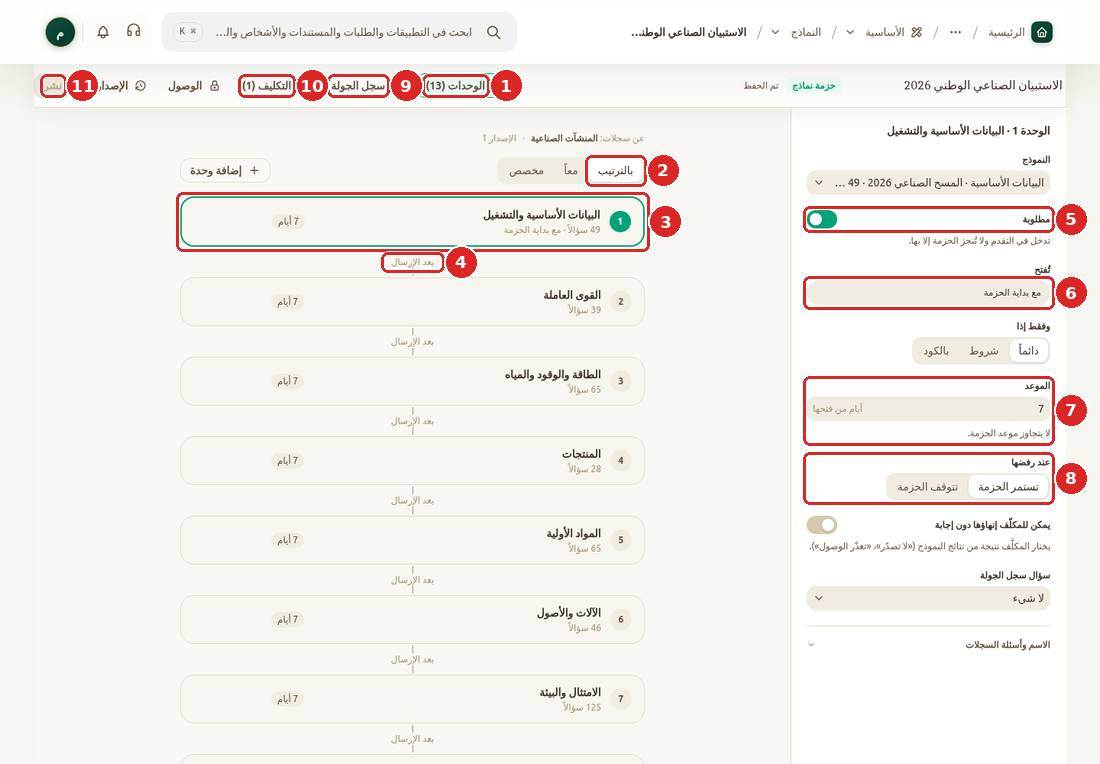
\includegraphics[width=\linewidth]{assets/screens/forms-package-ar.jpg}
\caption{حزمة نماذج ووحداتها}
\label{fig:forms-package}
\shotnote{تعرض الصورة حزمة فيها وحدات مرتبة، وإعدادات الوحدة المختارة في اللوحة الجانبية. تفيدك في ضبط ترتيب النماذج وشروط فتحها ومواعيدها قبل ربط الحزمة بخطة التكليف. ① «الوحدات». ② طريقة الفتح: «بالترتيب» أو «معاً» أو «مخصص». ③ بطاقة الوحدة الأولى. ④ «بعد الإرسال»: تُفتح التالية بعد إرسال السابقة. ⑤ «مطلوبة». ⑥ «تُفتح»: هنا «مع بداية الحزمة». ⑦ «الموعد» بالأيام. ⑧ «عند رفضها». ⑨ «سجل الجولة». ⑩ «التكليف»: الخطة التي توزع الحزمة. ⑪ «نشر».}
\end{figure}

\begin{rcnote}[تطبيق المثال: حزمة «مسح تشغيل الأفق»]
تنشئ سارة الحزمة وتختار «بالترتيب». الوحدة 1 «بيانات التشغيل»: مطلوبة، وتُفتح مع بداية الحزمة، وموعدها 7 أيام. الوحدة 2 «متابعة الاحتياج»: تُفتح بعد إرسال الوحدة 1، و«وفقط إذا» أيام التوقف أكبر من 0. في مثالنا أيام التوقف 3، فتُفتح الوحدة 2 لعمر. ولو كانت 0، لتُخطّيت الوحدة 2 واكتملت الحزمة بالوحدة الأولى. تفعّل سارة «سجل الجولة» ثم تنشر.
\end{rcnote}

\textbf{انتبه:} جمع النموذجين في حزمة لا ينقل الإجابات بينهما تلقائياً. فكل نموذج يقرأ من ملف المنشأة ويكتب فيه بحسب ربطه.

\begin{rcchecklist}[قبل ربط الحزمة بالخطة]
\begin{checklist}
\item «بيانات التشغيل» منشور، وأسئلته الخمسة وقواعده مجرّبة بالقيم 3 و0 و40.
\item سؤال «المنشأة» مفعّل فيه «سؤال سجل»، والإجابات تُكتب «عند الاعتماد».
\item «المسار» مفعّل في النموذجين، ومسار الموافقة: تدقيق آلي، ثم ليلى، ثم خالد، ثم رنا.
\item «متابعة الاحتياج» منشور، وفيه سؤال «المنشأة» نفسه.
\item الحزمة «مسح تشغيل الأفق» منشورة، و«سجل الجولة» مفعّل، والوحدة 2 شرطية.
\end{checklist}
\end{rcchecklist}

الحزمة جاهزة الآن. في الفصل~\ref{ch:05-plans} نربطها بخطة «متابعة تشغيل الأفق» ونطلق الجولة.
